%%%%%%%%%%%%%%%%%%%%%%%%%%%%%%%%%%%%%%%%%%%%%%%%%%%%%%%%%%%%%%%%%%
%%%%%%%% ICML 2013 EXAMPLE LATEX SUBMISSION FILE %%%%%%%%%%%%%%%%%
%%%%%%%%%%%%%%%%%%%%%%%%%%%%%%%%%%%%%%%%%%%%%%%%%%%%%%%%%%%%%%%%%%

% Use the following line _only_ if you're still using LaTeX 2.09.
%\documentstyle[icml2013,epsf,natbib]{article}
% If you rely on Latex2e packages, like most moden people use this:
\documentclass{article}

% For figures
\usepackage{multirow}

\usepackage{graphicx} % more modern
%\usepackage{epsfig} % less modern
\usepackage{subfigure} 

% For citations
\usepackage{natbib}

% For algorithms
\usepackage{algorithm}
\usepackage{algorithmic}

% As of 2011, we use the hyperref package to produce hyperlinks in the
% resulting PDF.  If this breaks your system, please commend out the
% following usepackage line and replace \usepackage{icml2013} with
% \usepackage[nohyperref]{icml2013} above.
\usepackage{hyperref}
\nocite{*}

% Packages hyperref and algorithmic misbehave sometimes.  We can fix
% this with the following command.
\newcommand{\theHalgorithm}{\arabic{algorithm}}

% jovo added stuff
\newcommand{\iid}{\overset{iid}{\sim}}
\newcommand{\mbX}{\mathbf{X}}
\newcommand{\mbY}{\mathbf{Y}}
\newcommand{\Real}{\mathbb{R}}
\providecommand{\mh}[1]{\hat{#1}}
\providecommand{\mb}[1]{\boldsymbol{#1}}
\providecommand{\mc}[1]{\mathcal{#1}}
\newcommand{\from}{{\ensuremath{\colon}}}           % :
\usepackage{amsmath,amssymb,amsfonts}

% Employ the following version of the ``usepackage'' statement for
% submitting the draft version of the paper for review.  This will set
% the note in the first column to ``Under review.  Do not distribute.''
\usepackage{icml2013} 
% Employ this version of the ``usepackage'' statement after the paper has
% been accepted, when creating the final version.  This will set the
% note in the first column to ``Proceedings of the...''
% \usepackage[accepted]{icml2013}


% The \icmltitle you define below is probably too long as a header.
% Therefore, a short form for the running title is supplied here:
\icmltitlerunning{Multiresolution dictionary learning for conditional distributions}

\begin{document} 

\twocolumn[
\icmltitle{Multiresolution dictionary learning for conditional distributions}

% It is OKAY to include author information, even for blind
% submissions: the style file will automatically remove it for you
% unless you've provided the [accepted] option to the icml2013
% package.

\icmlauthor{Francesca Petralia}{fp12@duke.edu}
\icmladdress{Department of Statistical Science, Box 90251, Duke University, Durham, North Carolina 27708, U.S.A.}
\icmlauthor{Joshua Vogelstein}{joshuav@jhu.edu}
\icmladdress{Department of Statistical Science, Box 90251, Duke University, Durham, North Carolina 27708, U.S.A.}
\icmlauthor{David B. Dunson}{dunson@stat.duke.edu}
\icmladdress{Department of Statistical Science, Box 90251, Duke University, Durham, North Carolina 27708, U.S.A.}

% You may provide any keywords that you 
% find helpful for describing your paper; these are used to populate 
% the "keywords" metadata in the PDF but will not be shown in the document
\icmlkeywords{Density regression; Dictionary learning, Manifold learning; Mixture of experts; Multiresolution stick-breaking; Nonparametric}

\vskip 0.3in
]

\begin{abstract} 
Nonparametric estimation of the conditional distribution of a response given high-dimensional features is a challenging problem.  In many settings it is important to allow not only the mean but also the variance and shape of the response density to change flexibly with features, which are massive-dimensional with a distribution concentrated near a lower-dimensional subspace or manifold.  We propose a  multiresolution model based on a novel stick-breaking prior placed on the dictionary weights.  The algorithm scales efficiently to massive numbers of features, and can be implemented efficiently with slice sampling.  State of the art predictive performance is demonstrated for toy examples and an important application to predicting drug response to anti-depressants.
\end{abstract} 

Key words: Density regression; Dictionary learning, Manifold learning; Mixture of experts; Multiresolution stick-breaking; Nonparametric 

\section{Introduction}

Massive datasets are becoming a ubiquitous by-product of modern scientific and industrial applications. These data present novel statistical and computational challenges for machine learning because many previously developed theoretical and methodological approaches do not scale-up well.  Specifically, these data are problematic because of their ultrahigh-dimensionality, and relatively low sample size (the ``large p, small n'' problem \cite{West}).
% Massive datasets arise from a variety of sources including neurological, image, video and biological applications. 
Parsimonious models for such ultrahigh-dimensional data assume that the density in the ambient dimension concentrates around a lower-dimensional (possibly nonlinear) subspace.  Indeed, a plethora of methodologies are emerging to estimate such lower-dimensional ``manifolds'' from high-dimensional data \cite{??}.  

We are interested in using such lower-dimensional embeddings to obtain estimates of the conditional distribution of some target variable(s).  This \emph{conditional regression} setting arises in a number of important application areas, including neuroscience, genetics, and video processing.  For example, one might desire a machine diagnosis for a patient presenting with a number of complicated psychiatric symptoms.   The challenge would then be to estimate the probability that the patient fits any of the diagnostic criteria for some category of mental illness via a $\mathcal{O}(10^6)$ dimensional image of the subject's brain. 


\section{Setting} % (fold)
\label{sec:setting}

Let $\mbX \from \Omega \to \mathcal{X} \subseteq \Real^D$ be a $D$-dimensional Euclidean vector-valued \emph{predictor} random variable.  Let $F_X$ denote the \emph{marginal} probability density of $\mbX$, and $f_X$ be the probability that  $\mbX=X \in \mc{X}$.  We assume that $F_X$ concentrates around a lower-dimensional (possibly nonlinear) subspace $\mc{M}=\{\mu \in \mc{M}\}$.  For example, $\mc{M}$ could be a union of affine subspaces, or a smooth compact Riemannian manifold, etc.  

Let $\mbY \from \Omega \to  \mathcal{Y} \subseteq \Real$ be a real-valued \emph{target} random variable. We further assume that \emph{conditional} distribution is a function of only the position of $X$ along the manifold, $F_{Y|X}=F_{Y|\mu}$. Let $X$ and $Y$ be sampled from some true but unknown joint distribution $(X,Y) \sim F_{X,Y}$.  Given a realization $X$ of predictors, we would like to know $F_{Y| \mbX=X}$.  

We obtain $\mh{F}_{Y|X}$---an estimate of this conditional density---via a \emph{point cloud}.  Specifically, we assume that we obtain $n$ independently and identically sampled observations, $(X_i,Y_i) \iid F_{X,Y}$, for $i \in [n]=\{1,2,\ldots,n\}$. 


% section setting (end)

\section{A Simple Illustrative Example} % (fold)
\label{sec:a_simple_illustrative_example}

Factorize the joint distribution $F_{X,Y}=F_X F_{Y|X}$.  Let $X$ live on some smooth one-dimensional Riemannian submanifold embedded in $\Real^D$.  Let $Y$ be a univariate Gaussian random variable whose mean and variance vary with the location of $X$ along its geodesic.  
See Figure \ref{fig:wave} for a graphical depiction. The color of the line indicates the position of $X$ along its geodesic, as well as the mean and variance of $Y$.
We can formalize this model as follows.
Define the marginal $F_X = \mc{N}(\psi(\mu_i),\sigma^2 \mb{I}_D)$, where $\Psi =\{ \psi \from \mc{M} \to \Real^D\}$, $\mu_i \in \mc{M}$, $\sigma \in \Real$, $\mc{I}_D$ is the $D\times D$ dimensional identity matrix, and $\mc{N}(\cdot,\cdot)$ indicates a Gaussian distribution.  Let $\mc{M}$ be a smooth compact Riemannian manifold, such as the oscillating D-wave.
% 
% One common model assumption is that each $X_i = \psi(\mu_i) + \epsilon_i$, where $\mu_i \in \mc{M}$, $\psi \from \mc{M} \to \mc{X}$, and $\epsilon_i \iid \mc{N}(\mb{0},\mb{\Sigma})$, with $\mb{0} \in \Real^D$ and $\mb{\Sigma}$ a $D \times D$ dimensional covariance matrix.
% 
Define the conditional $F_{Y|X} = \mc{N}( \mu_X, \mu_X)$.  




% section a_simple_illustrative_example (end)

\section{Approach} % (fold)
\label{sec:approach}



Our approach follows from assuming that the conditional distribution of the target variable is a simple function of a low-dimensional representation of the predictor variable (which lives in a high-dimensional ambient space).  We pursue a two-stage strategy.  In the first stage, we try to find a low-dimensional representation of the predictors via a multiscale nonlinear partitioning of the data.  In other words, we recursive partition $\{X_i\}=\{X_i\}_{i \in [n]}$ to obtain subsets of $\{X_i\}$ that are increasingly homogeneous according to some metric.  Thus, associated with each sample $i$ is a \emph{path} along the partition tree encoding to which child $i$ belongs in each scale of the tree.  

In the second stage, we estimate the conditional distribution of the target variable as a function of the multiscale embedding of the predictor

a few key insights. First, the target variable's distribution might be a simple function of a low-dimensional representation of the high-dimensional predictor variable.  


For example, $Y$ might be a Gaussian function whose mean and variance scale linearly according to a linear combination of a mixture of Gaussians


% dimensionality reduction and partitioning

With any dimensionality reduction technique comes an inherent \emph{bias-variance} tradeoff.  In particular, embedding in a lower-dimensional space potentially increases bias, but lowers variance.  The optimal bias-variance tradeoff depends jointly on the data and the exploitation task.  One strategy to combat this bias-variance tradeoff consists of obtaining a \emph{multiresolution} embedding.  In other words, one can estimate lower-dimensional subspaces within which the data concentrate at multiple scales.  (Bayesian) averaging across these scales can yield improvements in the inferential task.  


We proceed via a two-stage approach as a first attempt.  In the first stage, 


A simple and common strategy is to find a lower-dimensional linear or affine subspace for the predictor data.  Principal components analysis (PCA) \cite{Jolliffe} finds the optimal $k$-dimensional embedding for any $k < p$, where $p$ is the ambient dimension of the data.  Optimal here is defined as minizing the Frobenius norm error between the original data and the smoothed data (the lower-dimensional data projected back up to the higher-dimensional space).  

% reduced rank regression and sparse regression as special case of linear subspaces
% section approach (end)



In all these applications, common models utilized for density estimation, classification, variable selection and predictions fail to be efficient and cannot be applied. 
Dealing with large amounts of data requires the introduction of new models able to process the data accurately and efficiently. 
In this paper, we will focus on conditional density estimation for massive datasets. Conditional density estimation aims to estimates the density of the response $y \in \mathcal{Y}$ given a set of predictors $(x_1, x_2, \ldots, x_p)\in \mathcal{X}$. Though, a variety of flexible models have been proposed in the last decade, density estimation remains challenging for large sample sizes and high dimensional predictors. 

The need to deal with a large number of observations motivated the literature on divide-and-conquer techniques, a class of algorithms  extensively used in density estimation, classification and prediction. Well known examples are classification and regression trees (CART) \cite{CART} and multivariate adaptive regression trees (MARS) \cite{MARS}. These algorithms fit surfaces to data by explicitly dividing the input space into a nested sequence of regions, and by fitting simple surfaces  within these regions. Though these methods are appealing to reduce the dimensionality of the problem, single tree estimates are generally associated to high variance. A possible solution to this problem would be combining estimates resulting from different trees. Well known examples are bagging \cite{Bagging}, boosting \cite{Boosting} and random forest \cite{RandomForest}. Though these algorithms can substantially reduce the variance, they can be computationally intensive. 

Mixture of experts \cite{mixtureexperts} is another divide-and-conquer algorithm particularly useful to reduce the variance associated to single tree estimates. As opposed to other divide-and-conquer algorithms, mixture of experts rely on soft partitioning algorithms that allows  observations to lie simultaneously in different subsets. A mixture of experts model is a mixture model in which the model parameters, including mixture weights, are functions of covariates. Several mixture of experts models have been proposed in the last twenty years. some of them gain flexibility by dealing with infinitely many experts \cite{infiniteMoE}  \cite{AltInfMoE}, others propose a hierarchical structure where a mixture model is fit in each subset  \cite{HierMoF} \cite{BHierMoF}.  

A significant downside of all divide-and-conquer algorithms is their poor scalability to high dimensional predictors. As the number of features increases, the problem of finding the best splitting attribute becomes intractable so that CART, MARS and multiple trees models cannot be efficiently applied. Also mixture of experts models become computationally demanding, since both mixture weights and dictionary density are predictor dependent. In an attempt to make mixture of experts more efficient sparse extensions relying on different variable selection algorithms have been proposed \cite{SparseMoF}. However, performing variable selection in high dimensions is still a challenging problem, especially when multiple parameters involved in the model, such as weights and mean functions, depend on high dimensional predictors.

 In order to efficiently deal with massive datasets, we propose a novel multiresolution approach which starts by learning a multiscale dictionary of densities, constructed as Gaussian within each set of multiscale partition tree for the features. The proposed approach is based on a two-stage algorithm where first the predictor space is recursively partitioned and then, considering the partition as fixed, a multiresolution stick-breaking process is estimated. According to the proposed process, observations can lie simultaneously in subsets located at different resolution levels. This results in a model that allows borrowing information across different resolution levels and reaches a good compromise in terms of the bias and variance trade-off. The tree partition is found by implementing a fast multiscale technique used for graph partitioning \cite{metis}.  We show that the algorithm scales efficiently to massive numbers of features, and can be implemented efficiently with gibbs sampling.  State of the art predictive performance is demonstrated for toy examples and an important application to predicting drug response to anti-depressants.

 
 
\section{Model Specification}

\subsection{ Model Structure} %In order to deal with massive datasets, efficient and scalable statistical models  need to be introduced. 
This paper will mainly focus on the problem of estimating the conditional density $f(y|x)$ of the response given a high dimensional vector of predictors, concentrated near a lower-dimensional subspace $\mathcal{M}$ embedded in $\mathcal{X}$. In dealing with massive datasets, the idea of combining different local models defined on subsets of the predictor space have increased popularity in the last decade. These methods, generally known as divide-and-conquer algorithms, aim to replace complicated conditional density functions with a combination of simple densities defined locally, on subsets of the predictor space.

Suppose we define a multiscale partition of $\mathcal{X}$.  Generation one corresponds to the entire $\mathcal{X}$ denoted as $\mathcal{X}^1$.  At generation two, $\mathcal{X}^1$ is split into two mutually exclusive partition sets, $\mathcal{X}^1=\left(\mathcal{X}^2_1, \mathcal{X}^2_2\right)$. Each subset is recursively partitioned into two subsets so that for a general partition level $\ell$ the partition will be given by $\mathcal{X}^{\ell}=\left(\mathcal{X}^{\ell}_1, \ldots, \mathcal{X}^{\ell}_{2^{\ell-1}}\right)$. Let us assume this process proceeds for $k$ levels. Let $(\ell,s)$ be the node associated to the $s$th subset at resolution level $\ell$. Let $ch(\ell,s)$ and $pa(\ell,s)$ be respectively the set of children and parents of node $(\ell, s)$. Let $A_{\ell}(x) \in \{1, \ldots, 2^{\ell-1}\}$ be the location of predictor $x$ at level $\ell$, with $A_1(x)$ equal to 1 by definition. 

We characterize the conditional density $f(y|x)$ as a convex combination of multiscale dictionary densities.  At level one, the global parent density is denoted $f_1$. The dictionary density at generation $j$ is $f_{B_j}$ with $B_j=\{j,A_j\}$, for $j=2,\ldots, k$. Then, $f(y|x)$ is defined as the convex combinations of densities $\{f_{B_j}\}_{j=1}^k$ with weights $\{\pi_{B_j(x)} \}_{j=1}^k$, i.e.
\begin{eqnarray}
f(y|x) = \sum_{j=1}^k \pi_{B_j(x)} f_{B_j(x)}(y),  \label{eq:base}
\end{eqnarray}
where $0 \le \pi_{B_j(x)} \le 1$ and $\sum_{j=1}^k \pi_{B_j(x)}=1$.

Each $B(x)$ is a set encoding the path through the partition tree up to generation $k$ specific to predictor value $x$. According to model \ref{eq:base}, one observation can simultaneously lie in subsets located at different resolution levels. This is particularly useful to reach a good compromise between the bias and variance trade-off as explained in the next section.  Moreover, it allows borrowing information across different resolution levels. Though the proposed approach reminds a mixture of experts model \cite{mixtureexperts}, the two approaches are  completely different since under (\ref{eq:base}) neither mixture weights nor dictionary densities directly depend on predictors. This allows our model to scale efficiently to high dimensional predictors.

Now let us examine the implications of model (\ref{eq:base}). For two predictor values $x$ and $x'$ located close together, it is expected that the paths will be similar, which leads to similar weights on the dictionary densities.  In the extreme case in which $x$ and $x'$ belong to the same leaf partition set, we have $B(x) = B(x')$ and the path through the tree will be the same.  Moreover, in this case, we will have $f(y|x)=f(y|x')$ so that up to $k$ levels of resolution the densities $f(y|x)$ and $f(y|x')$ are identical.  If the paths through the tree differ only in the final generation or two, the weights will typically be similar but the resulting conditional densities will not be identical. 

To derive mixture weights, a natural choice corresponds to a stick-breaking process \cite{stickbreaking}.  For each node $B_j(x_i)$ in the binary partition tree, define a stick length $V\{B_j(x_i)\} \sim \mbox{beta}(1,\alpha)$.  The parameter $\alpha$ encodes the complexity of the model, with $\alpha = 0$ corresponding to the case in which $f(y|x) = f(y)$.  We relate the weights in (\ref{eq:base}) to the stick-breaking random variables as follows: 
\begin{eqnarray*}
\pi_{B_j(x)} = V\left\{B_j(x)\right\} \prod_{B_h \in pa\left\{B_j\right\}} \left[1 - V\left\{B_h(x)\right\}\right],
\end{eqnarray*}
with $B_j(x)=\{j,A_j(x)\}$ and $V\{B_k(x)\}=1$ to ensure that $\sum_{j=1}^k \pi_{B_j}(x) = 1$.    
\vskip 12pt

\subsection{Theoretical properties} 

\section{Estimation}

The proposed approach is based on a two-stage algorithm where first the predictor space is recursively divided in different subsets using an efficient partitioning algorithm and then, considering the partition as fixed, a multiresolution stick-breaking process is estimated.  The predictor space is partitioned applying metis \cite{metis}, a fast multiscale technique used for graph partitioning. Though more complicated densities can be considered, dictionary densities $f_{B_j}$ will be estimated by assuming a normal form. In particular, densities corresponding to a particular partition set will be estimated considering observations for all subjects having predictors in that partition set. To be specific, for estimating density $f_{B_j}(y)$, we use the data $\{ y_i: x_i \in \mathcal{X}^j_{A_j} \}$. We then conduct the analysis treating the dictionary elements and partition sets as fixed and placing a prior on the weights $\pi_{B_j}$. 

Parameters involved in the dictionary density can be estimated using either frequentist or bayesian methods. Both methodologies have advantages and disadvantages. The frequentist approach, relying on maximum likelihood estimation, would allow to obtain parameter estimates in a faster and more efficient way. On the other hand, bayesian methods can avoid singularities associated with traditional maximum likelihood inference. 

In any case, inference on stick breaking weights will be carried out using the Gibbs sampler. For this purpose, introduce the latent variable $S_i \in \{1,\ldots,k\}$, for $i=1,\ldots,n$, denoting the multiscale level used by the $i$th subject. Let $n(B_j)$ be the number of observations allocated to node $B_j$. Then, at each gibbs sampling iteration, stick breaking are sampled as follows 
\begin{enumerate}
\item Update $S_i$ by sampling from the multinomial full conditional with 
\[\mbox{Pr}( S_i = j\, |\, -) = \frac{ \pi_{B_j(x_i)}f_{B_j(x_i)}(y_i) }{ \sum_{h=1}^k \pi_{B_h(x_i)}f_{B_h(x_i)}(y_i) } \label{eq:prS}\]
\item Update stick-breaking random variable $V_{B_j(x_i)}$, for $j=1, \ldots, k$ and $i=1, \ldots, n$, from $Beta(a_p,b_p)$ with $a_p=1+n\left\{B_j(x_i)\right\}$ and $b_p=\alpha+\sum_{B_h(x_i) \in ch\{B_j(x_i)\}} n\left\{B_h(x_i)\right\}$.
\end{enumerate}

\section{Simulation Studies}


In order to assess the predictive performance of the proposed model, different simulation scenarios were considered. Let $n$ be the number of observations, $y$ the response variable and $x \in \mathcal{R}^p$ a set of predictors. In order to sample stick breaking weights, the Gibbs sampler was run considering $20,000$ as the maximum number of iterations with a burn-in of $1,000$. Gibbs sampler chains were stopped testing normality of normalized averages of functions of the Markov chain \cite{Chauveau98anautomated}. 

In all examples below, predictors were assumed to belong to a lower dimensional manifold. In the first three simulation studies, the manifold was assumed to be a lower dimensional plane. In particular, the vector of predictors was modeled through a factor model, i.e. $x_i=\Lambda \eta_i + \epsilon_i$ with $\epsilon_i \sim N(0,I)$, $\Lambda$ being a $(p \times k)$ matrix, $\eta_i$ a $k$ dimensional vector with elements drawn from a standard nromal and $k<<p$. The response $y$ was assumed to be a function of the latent variable $\eta$ so that  the dependence between response and predictors was induced by the shared dependence on the latent factors.  In all examples, $\Lambda$ was assumed to be a sparse matrix with level of sparsity increasing with the number of columns and non zero elements of $\Lambda$ drawn from a standard normal density. In the fourth simulation study, predictors were drawn from the swiss roll manifold.

In the first simulation study, $(k,p)$ were chosen to be $(5,1000)$ and response and predictors were jointly sampled from the above factor model.  In the second simulation study, $(k,p)$ were chosen to be $(5,10000)$ and the response was drawn from a $N(2,1)$ with probability $p=\exp\{\eta_1)/(1+\exp(\eta_1)\}$ and from a $N(-2,1)$ with probability $1-p$.  In the third simulation study, $(k,p)$ were chosen to be $(5,5000)$ and the response was drawn from a normal with mean and variance depending on the first latent factor as follows $y \sim N\{\eta_1^2-\eta_1^3, \exp(1-\eta_1)\}$.

Table \ref{table1} shows mean squared errors based on leave-one-out predictions under multiscale stick breaking, CART and lasso. In the first example, where a linear relationship is assumed between response and predictors, lasso performs better than CART. Instead, our approach is able to perform well in both linear and non linear case.  Figure 2 [coming soon] shows a plot of CPU usage under all three approaches as the number of predictors increases. Clearly, our multiscale stick breaking scales substantially better to massive number of features. 

It is important to note that under the proposed approach an estimate of the predictive densities of the data can be obtained. Figure \ref{plotDensity} shows the estimated density of two observations sampled from the second example. Clearly, as the number of observations in the training set increases, the two densities become closer to the true one. [will provide $95\%$ intervals, need to rerun codes] 
	

\begin{table}[t]
\caption{Mean and standard deviations of squared error under multiscale stick-breaking (MSB), CART and Lasso for sample size 50 and 100}
\label{table1} \vskip 0.15in \begin{center} \begin{small} \begin{sc}
\begin{tabular}{llllllllllllllllll}
\hline
\abovespace\belowspace
 sim &model& \multicolumn{2}{c}{mse}& \multicolumn{2}{c}{var}\\
 $n$&& 50 &100 &50 &100\\
\hline
\\
(1)&msb&   1.02 &  1.09 &1.26  &  1.68\\
&cart&  2.69&  2.29& 3.00 &    2.82\\
&lasso &  1.02 &   1.09 &  1.25&   1.66\\
\\
(2)&msb&0.56&0.55& 0.66&0.86\\ %normal3
&Cart& 0.67&0.55& 1.09&0.62\\
&Lasso& 0.84&0.99& 0.79&0.79\\

\\
(3)&msb&    0.89 &  0.78 &2.34  &  1.99\\
&cart&  1.25 &  0.83& 1.78 &    2.16\\
&lasso &   1.00 &   0.84 &    2.41&   2.00\\
\\
(4)
&msb& 0.89&0.71&3.30&4.20\\
&cart & 1.77 &1.24& 5.23&4.63\\
&lasso & 1.38 &0.79&3.29&4.49\\
\hline

\end{tabular}
\end{sc}
\end{small}
\end{center}
\vskip -0.1in
\end{table}


\begin{figure}
\centering
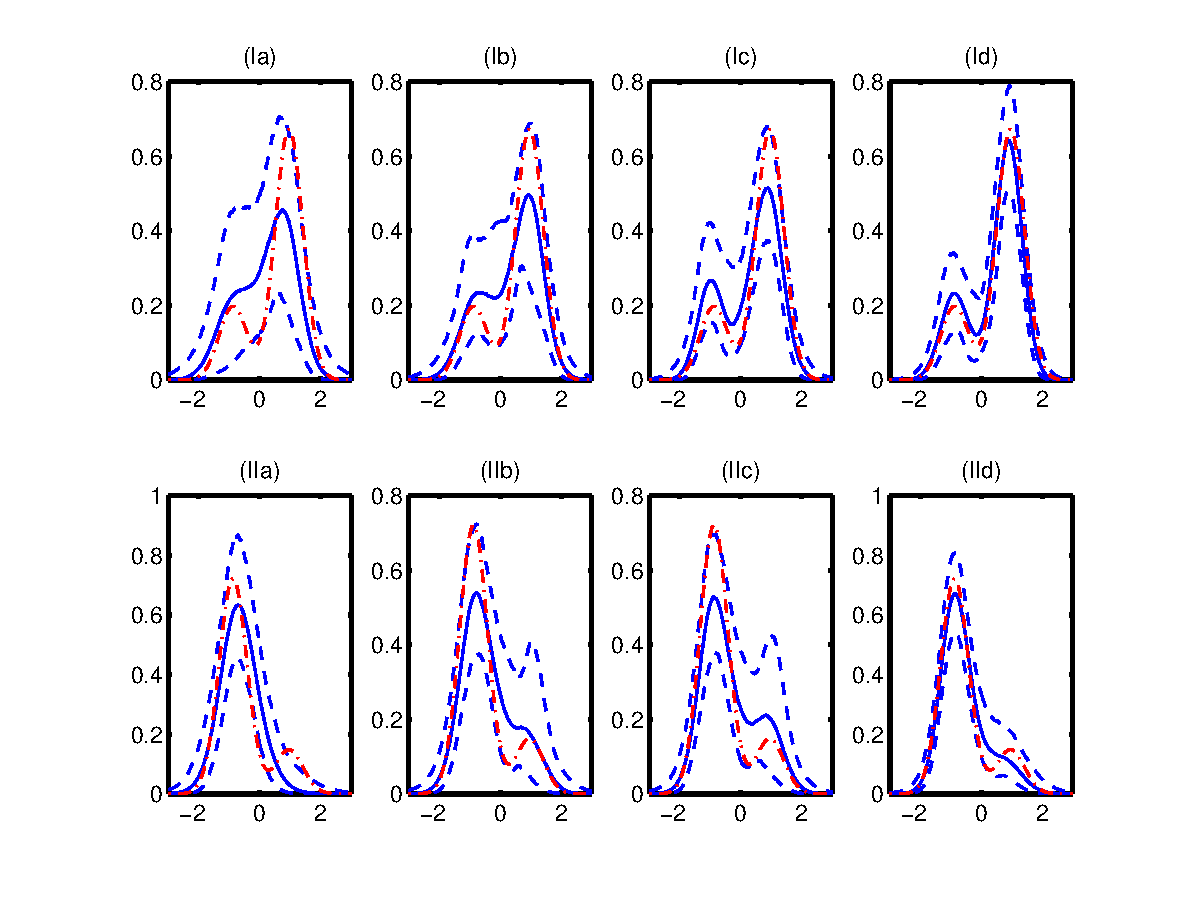
\includegraphics[scale=0.5]{figure2.eps}
\caption{Plot of true density (dashed-dotted line) and estimated density ($50$th percentile: solid line, $2.5$th and $97.5$th percentiles: dashed lines) for two observations $(I, II)$ considering different training set size (a:50, b:100, c:150, d:200). } \label{plotDensity}
\end{figure}


\section{Real data examples}

We assessed the predictive performance of the proposed method on a real dataset. This dataset consists of a measurement of creativity observed for $108$ subjects. We would like to predict the value of creativity based on the number of connections between different cortical regions of the brain. For each subject, we observe a brain graph consisting of $70$ cortical regions whose centers are depicted as vertices. Therefore, the brain graph involves $4,900$ vertices and $2,415$ different pairs of vertices. The vector of covariates consists in the logarithm of the total number of connections between all pairs of vertices. Both response and covariates have been normalized by subtracting the mean and dividing by the variance. The same Gibbs sampler as in section 4 was  utilized.

Table \ref{table3} shows mean and variance squared error based on leave-one-out predictions for CART, random forest, lasso and our approach. Variable $t_{T}$ is the amount of time necessary to obtain predictions for all subjects, while variables $t_M$ and $t_V$ are the mean and variance of time necessary to obtain prediction for one subject. Though CART is associated to a lower CPU time, it performs worse than all other approaches in terms of mean squared error. 


\begin{table}[t]
\caption{Mean and standard deviations of squared error under multiscale stick-breaking (MSB), CART, Lasso and random forest (RF)}
\label{table3} \vskip 0.15in \begin{center} \begin{small} \begin{sc}
\begin{tabular}{llllllllllllllllll}
\hline
\abovespace\belowspace
&msb&cart & lasso & rf\\
\hline
mse&   1.00 & 1.99 &1.10 & 1.09\\
 var& 1.42  & 3.23& 1.43& 1.54\\

\end{tabular}
\end{sc}
\end{small}
\end{center}
\vskip -0.1in
\end{table}


\newpage
\nocite{langley00}

\bibliography{multiscale5}
\bibliographystyle{icml2013}



\end{document} 

